Ce chapitre décrit les différents éléments mis en place pour chaîner les services afin d'obtenir une pipeline de génération de covers. En plus de ces derniers, le projet comprend un orchestrateur et une webapp. Le premier fait le lien entre la sortie d'un service et l'entrée du suivant et le deuxième permet de visualiser les résultats intermédiaires et finaux.

\section{Orchestrateur}

L'orchestration des différents services est l'élément central qui permet de lier ces derniers entre eux. Lors de la rédaction du cahier des charges \cite{CDC}, la proposition était d'utiliser l'outil Prefect\cite{prefect} qui permet la construction, le déploiement, la surveillance et l'orchestration de pipelines de données. 
Cependant, lors des premiers tests d'implémentation, il s'est avéré que cet outil était trop complexe pour les besoins du projet. En effet, dans le cadre de ce travail, la pipeline implémentée est simple et son exécution consiste uniquement à lancer les services les uns après les autres en envoyant des requêtes HTTP tout en transmettant les données de sortie d'un service à l'entrée du suivant.
Le choix se porte donc sur le développement d'un orchestrateur personnalisé afin d'éviter d'ajouter de la complexité là où il n'y en a pas besoin. Dans une optique de respect des spécification du CSIA-PME, FastAPI\cite{fastapi} qui permet de créer, gérer et exécuter des pipeline en liant les appels aux différents services est utilisé.

Une solution utilisant Prefect est également implémentée. Cependant, elle n'est pas utilisée de manière concrète dans le projet étant donné que cela demande de faire de nombreuses modifications sur la webapp et sur les différents services. Il est toutefois possible d'exécuter une pipeline avec Prefect en utilisant l'interface web proposée par l'outil.

\subsection{Orchestrateur FastAPI}

Afin d'orchestrer l'appel aux différents services, un système de gestion de pipeline est mis en place et s'utilise via des routes HTTP illustrées dans la figure \ref{fig:orchestrator_routes}. Ce système permet de gérer plusieurs pipelines en les plaçant dans une file d'attente et en les exécutant lorsque l'orchestrateur est disponible. Les diagrammes  \ref{fig:state_diagram} et \ref{fig:seq_diagram} illustre de manière détaillée les différents statuts possibles d'une pipeline et les différentes interactions de la création à l'obtention du résultat.

\begin{figure}[H]
    \begin{center}
        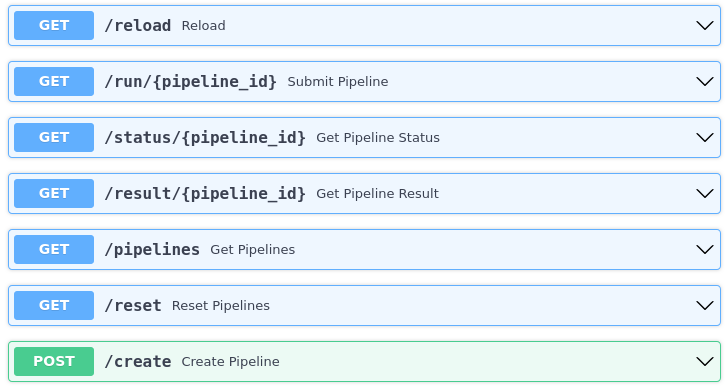
\includegraphics[height=5cm,]{rapport_PI/rsc/fastapi_orchestrator_routes.png}
        \caption{Routes exposées par l'orchestrateur FastAPI}
        \label{fig:orchestrator_routes}
    \end{center}
\end{figure}

\subsubsection*{Création d'une pipeline}
La première étape consiste à créer une nouvelle pipeline avec la route \textit{/create} avec soit un fichier audio au format MP3 ou OGG soit l'URL d'une vidéo Youtube en paramètre.
Une pipeline est créée avec le statut \textit{CREATED} et l'orchestrateur renvoie son identifiant.
Si un fichier audio est passé en paramètre alors ce dernier est sauvegardé et le chemin du fichier audio est associé à la pipeline et s'il s'agit de l'URL d'une vidéo Youtube, le lien uniquement est associé.

\subsubsection*{Soumission de la pipeline dans une file d'attente}
Dès que la pipeline est créée, il faut demander son exécution avec la route \textit{/run} en indiquant son identifiant en paramètre. L'orchestrateur change alors le statut pour \textit{WAITING} ce qui signifie que la pipeline est en attente d'être exécutée.

\subsubsection*{Exécution des différents services}
L'exécution effective des différentes pipelines est effectuée par un thread qui va sélectionner la première pipeline de la file d'attente avec le statut \textit{WAITING}.

La route \textit{/status} permet d'obtenir le statut d'une pipeline mais afin d'éviter un nombre de requête important, un WebSocket est mis en place pour permettre à la web app d'être informée lorsque la pipeline change d'état.

Si l'URL d'une vidéo YouTube a été fournie lors de la création de la pipeline, l'orchestrateur appelle le micro-service \textit{Youtube downloader} et stocke le résultat dans un fichier audio qui est associé à la pipeline. 

L'orchestrateur exécute ensuite les différents micro-services l'un après l'autre. Si l'exécution de l'un d'eux échoue, alors le statut de la pipeline passe à \textit{FAILED} et son exécution est interrompue. Les résultats intermédiaires ainsi l'état de la pipeline (\textit{RUNNING\_WHISPER}, \textit{RUNNING\_SENTIMENT}, \textit{RUNNING\_MUSIC\_STYLE}, \textit{RUNNING\_IMAGE\_GENERATION}) sont envoyé au WebSocket à chaque fois qu'un micro-service est exécuté. Cela permet à la web app d'informer l'utilisateur de l'état d'avancement et d'afficher les résultats intermédiaires.

\subsubsection*{Récupération des résultats}
Une fois que tous les micro-services ont été exécutés, le statut de la pipeline passe à \textit{RESULT\_READY}. 
La web app récupère ensuite les 3 images générées avec la route \textit{/result} en indiquant une nouvelle fois l'identifiant de la pipeline. Le statut de cette dernière est mis à jour et passe à \textit{FINISHED} ce qui indique à l'orchestrateur qu'il peut supprimer le fichier audio d'entrée ainsi que les fichiers de résultats associés.

\begin{figure}[H]
    \begin{center}
        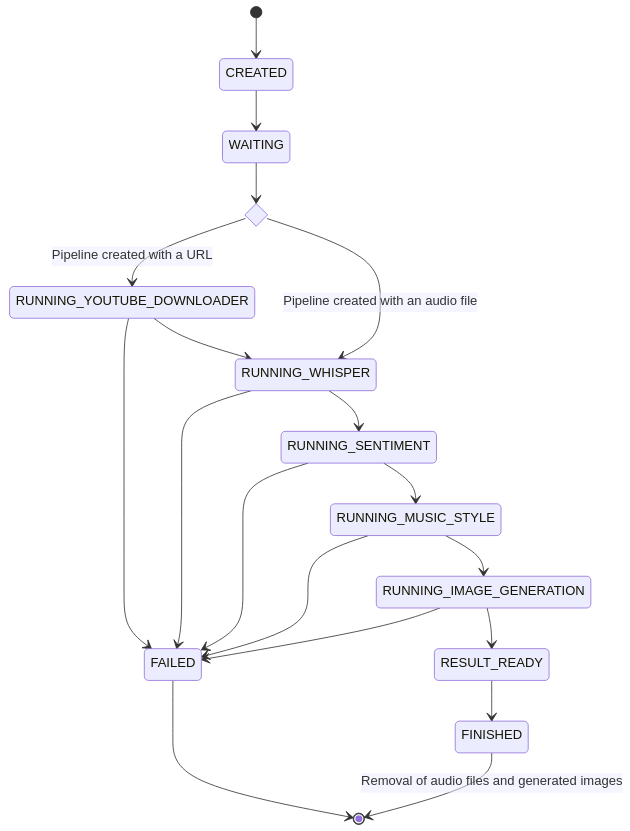
\includegraphics[height=23cm,]{rsc/orchestrator_state_diagram.png}
        \caption{Diagramme d'état d'une pipeline}
        \label{fig:state_diagram}
    \end{center}
\end{figure}

\begin{figure}[H]
    \begin{center}
        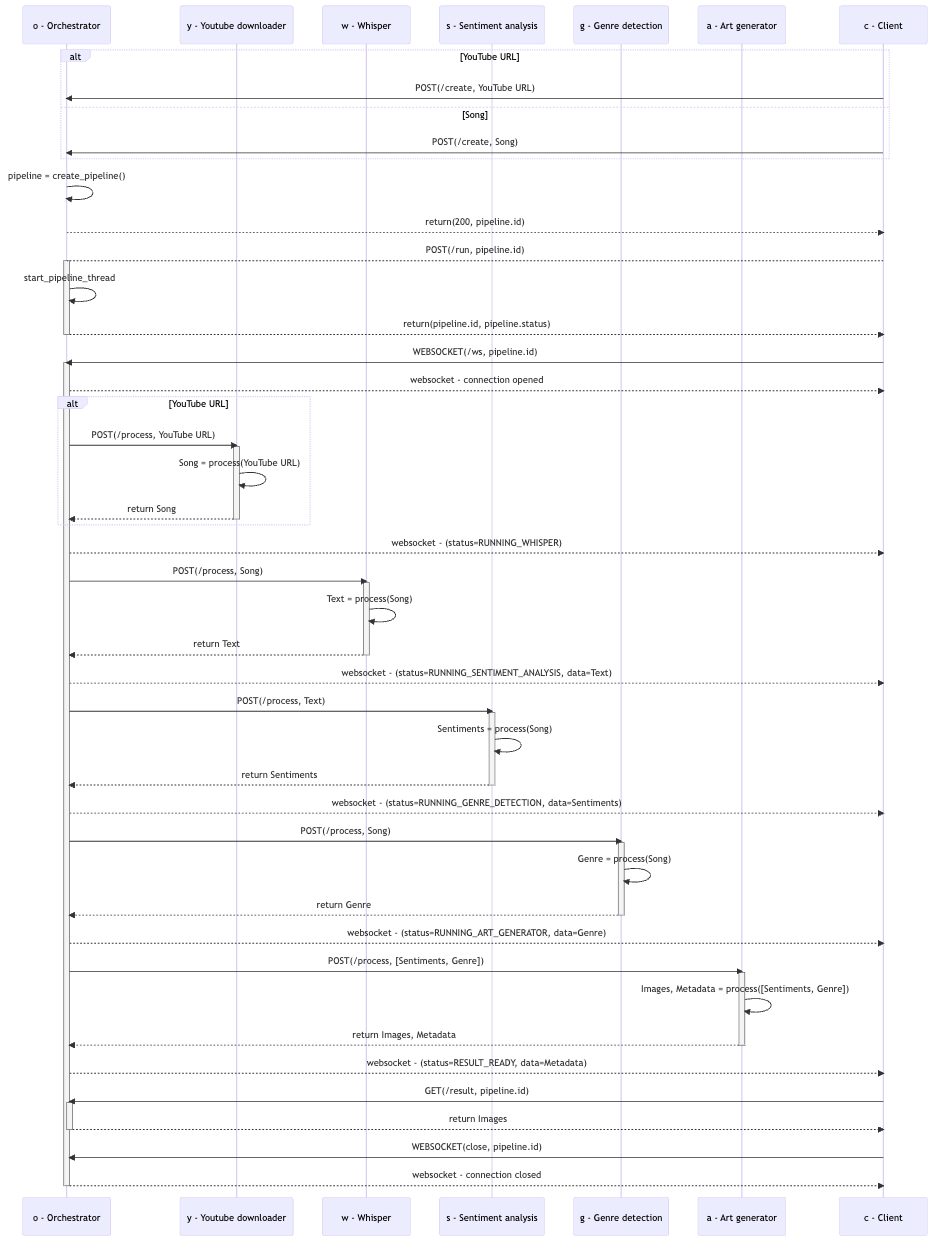
\includegraphics[height=23cm,]{rsc/sequence_diagram.png}
        \caption{Diagramme de séquence d'une exécution de pipeline}
        \label{fig:seq_diagram}
    \end{center}
\end{figure}

\section{Application web}
Afin de visualiser les différentes étapes et les résultats de notre pipeline, une application web est développée. Pour respecter les objectifs définis dans le cahier des charges \cite{CDC}, cette dernière est implémentée à l'aide de VueJS \ref{fig:webapp}.

\begin{figure}[H]
    \begin{center}
        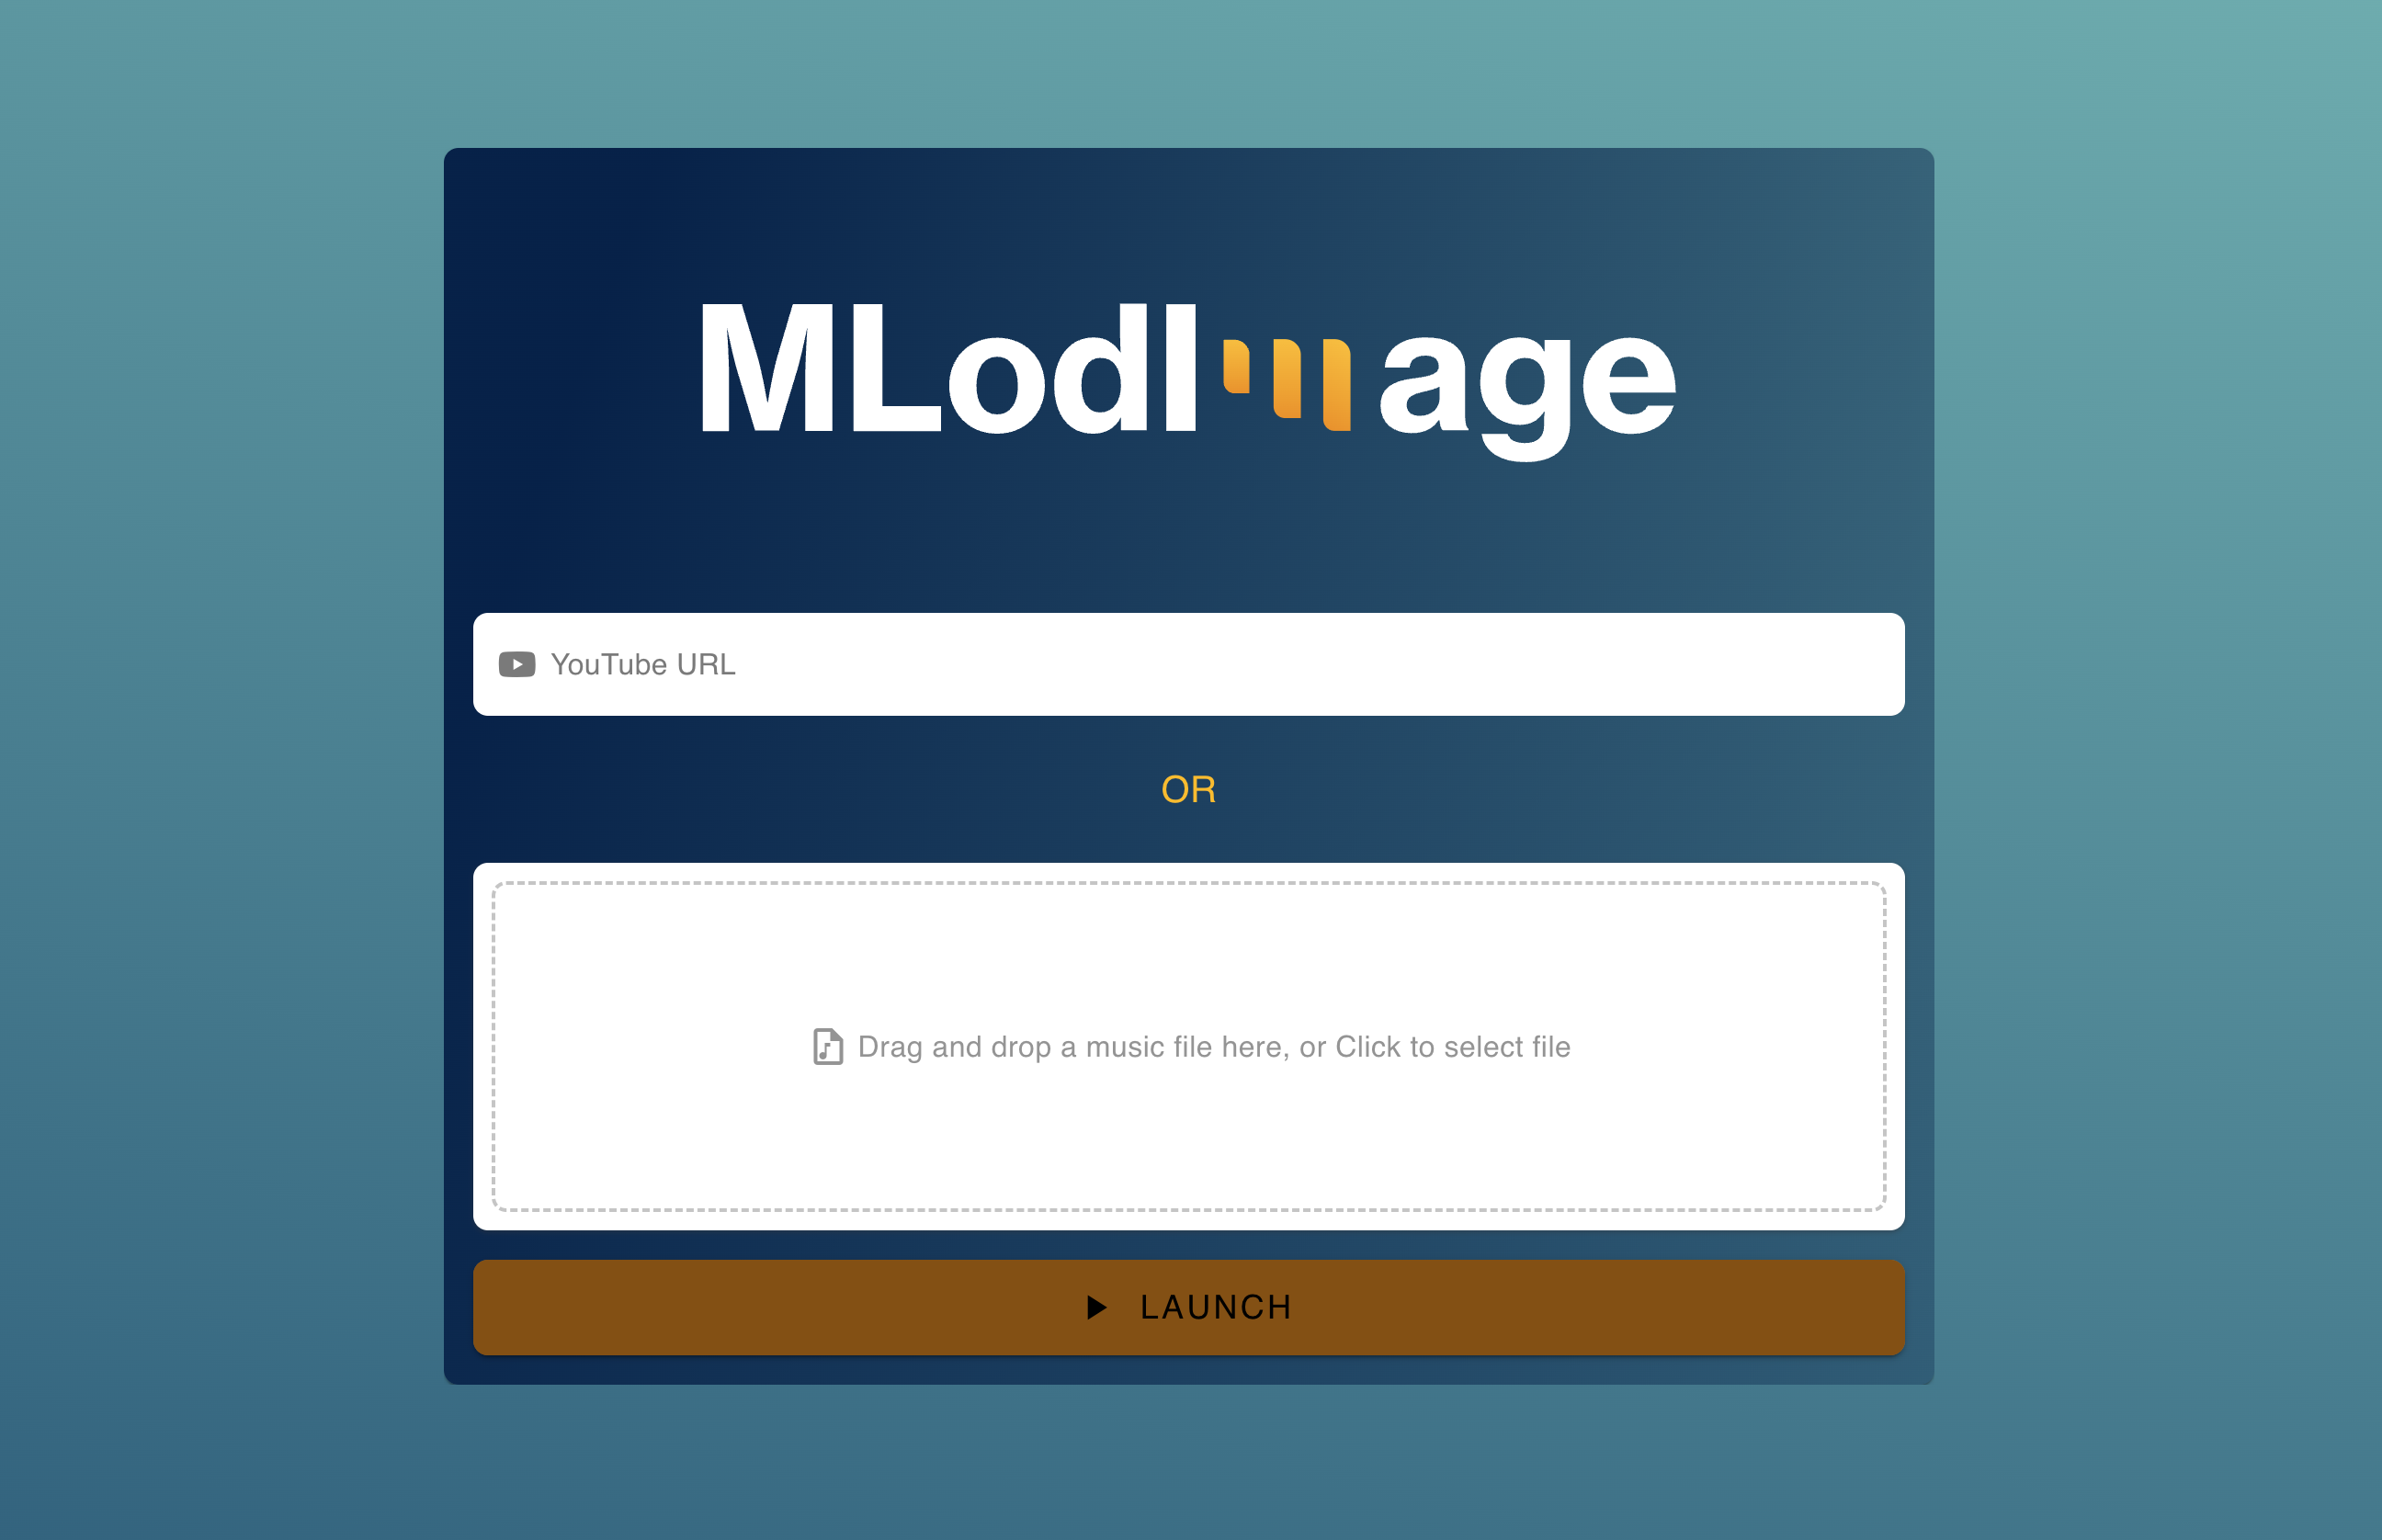
\includegraphics[width=10cm,]{rsc/webapp.png}
        \caption{Web app}
        \label{fig:webapp}
    \end{center}
\end{figure}

Le frontend dispose d'une interface qui permet, soit d'utiliser l'URL de YouTube, soit de glisser et déposer un fichier audio (figure \ref{fig:webapp_file_url}).

\begin{figure}[H]
    \begin{center}
        
\includegraphics[width=17cm,]{rapport_PI/rsc/webapp_file_url.png}
        \caption{Web app - YouTube URL (gauche) \& Fichier (droite)}
        \label{fig:webapp_file_url}
    \end{center}
\end{figure}

En lançant l'exécution, l'utilisateur peut suivre la progression à l'aide des messages de statut (figure \ref{fig:webapp_steps}).

\begin{figure}[H]
    \begin{center}
        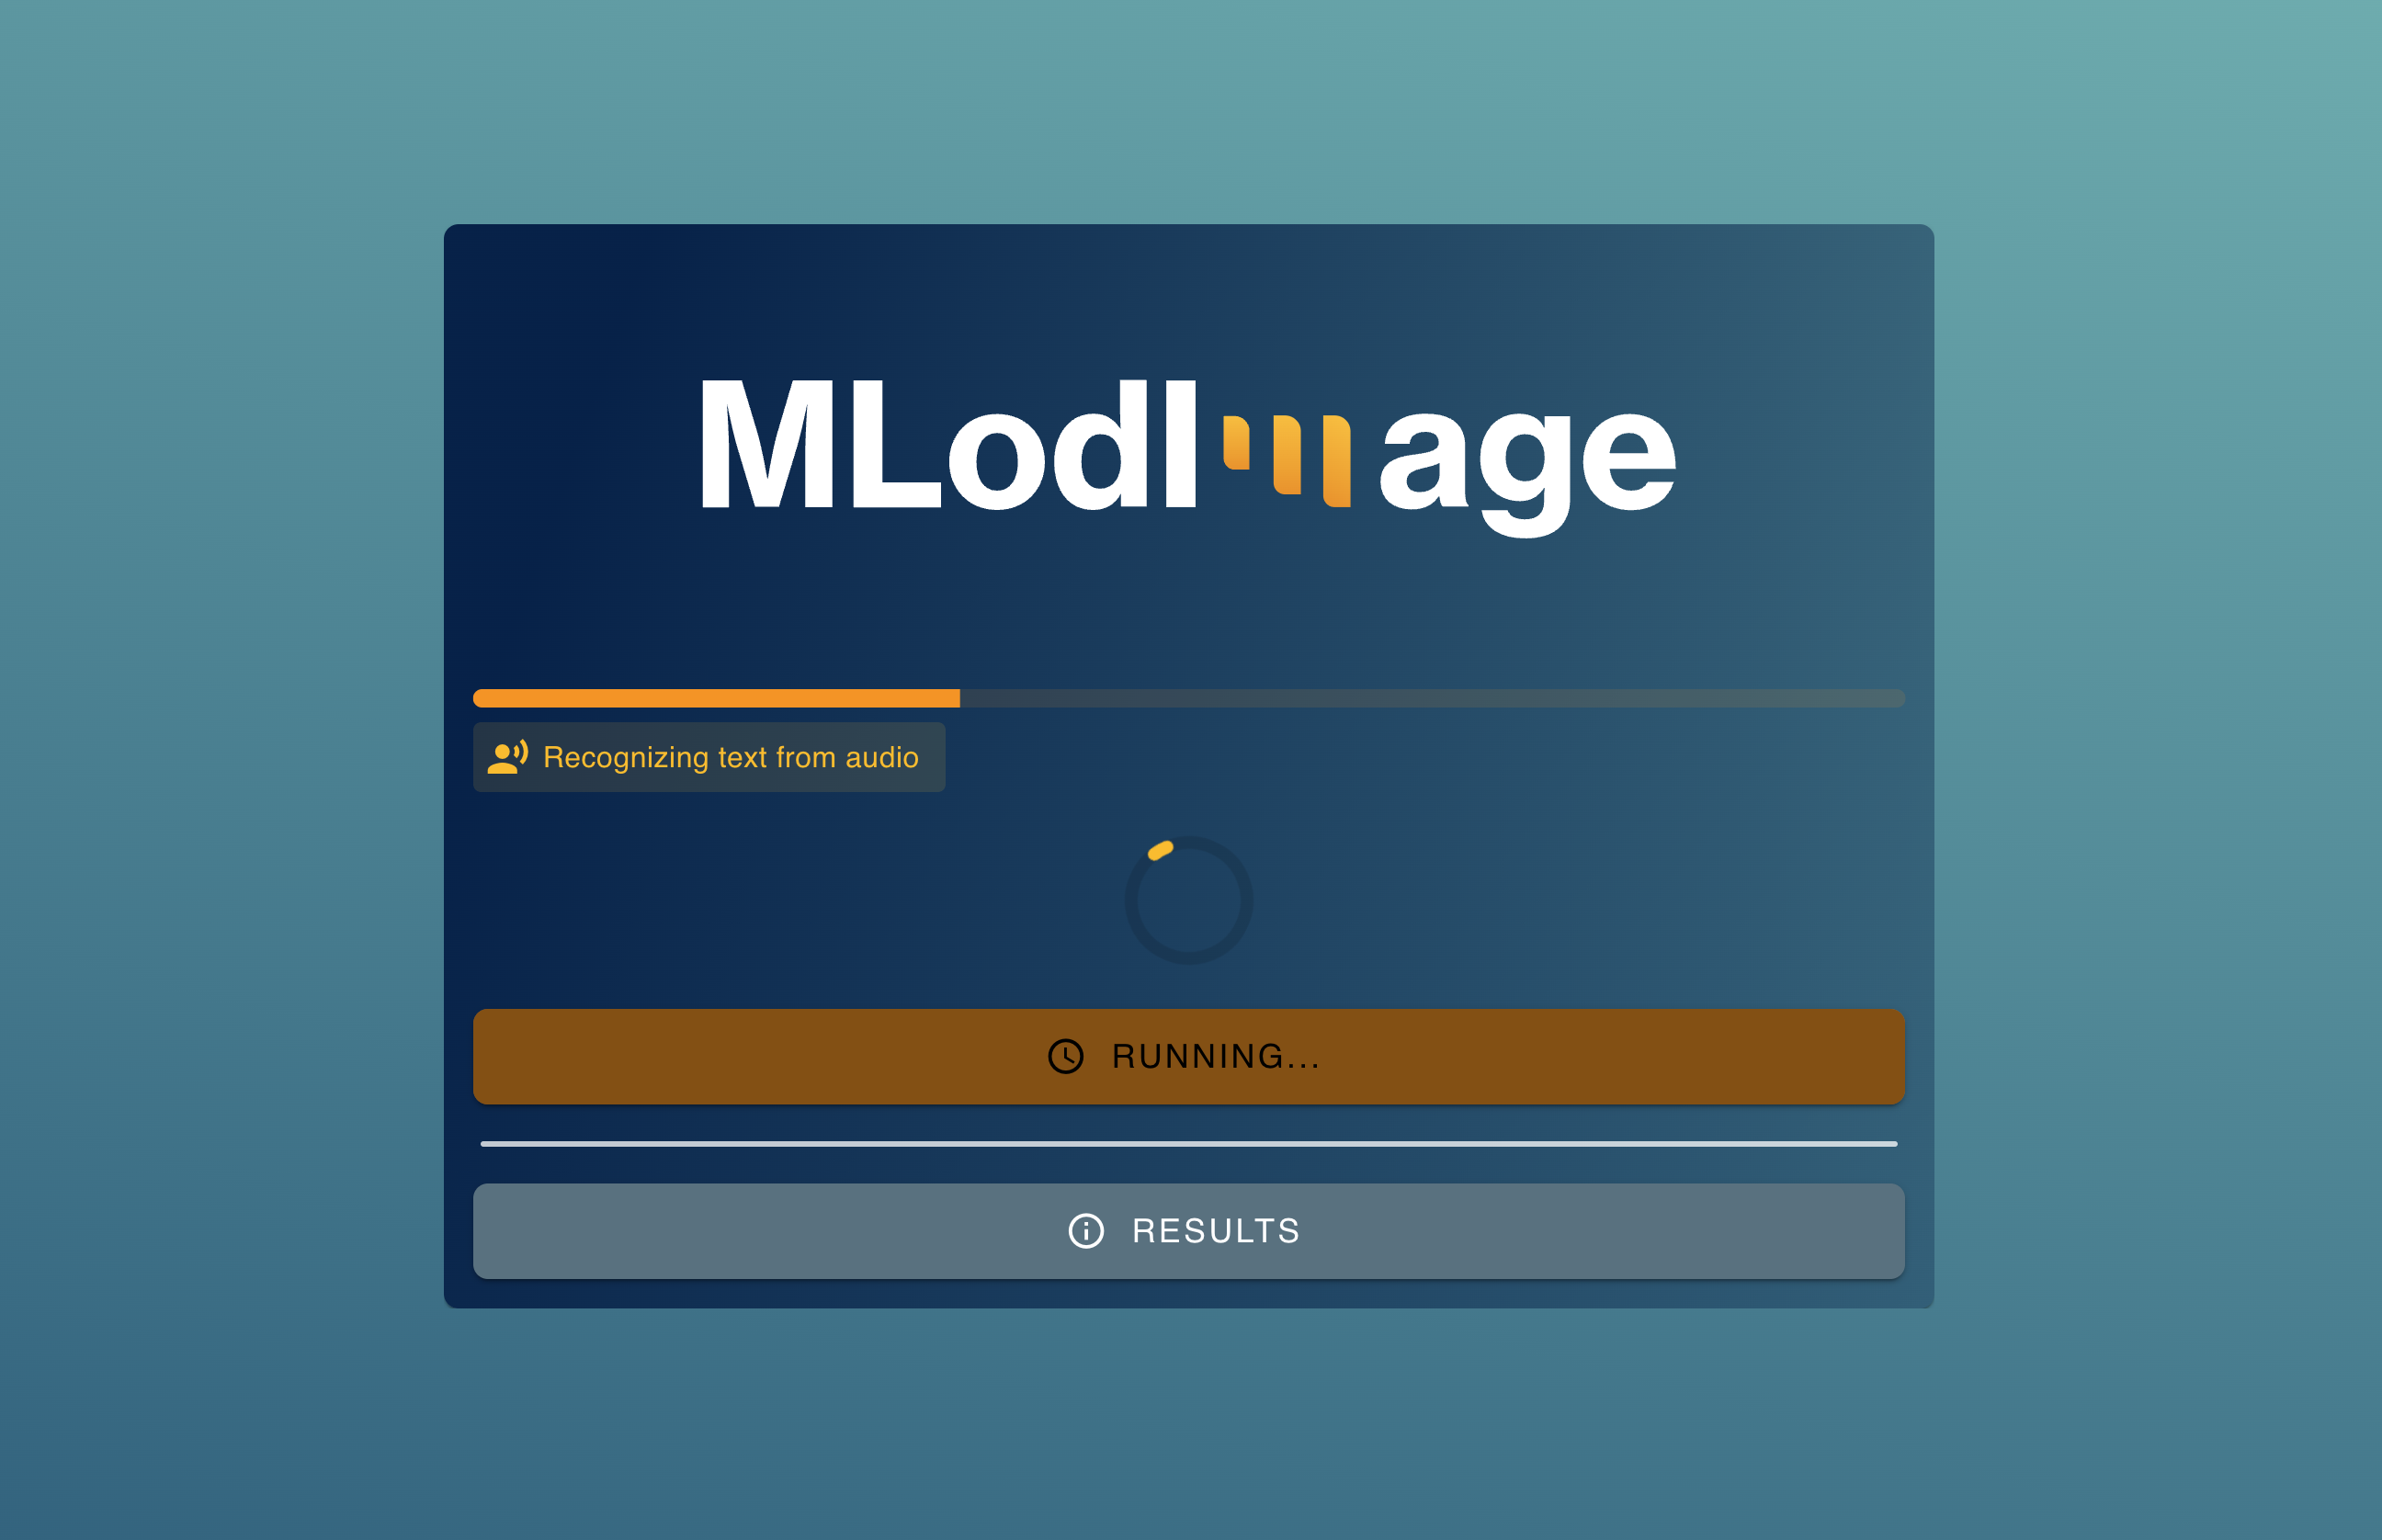
\includegraphics[width=10cm,]{rapport_PI/rsc/webapp_steps.png}
        \caption{Web app - Exécution}
        \label{fig:webapp_steps}
    \end{center}
\end{figure}

Grâce à la connexion via WebSocket, il est possible de recevoir les résultats intermédiaires. Pour les afficher, on peut cliquer sur le bouton dédié et une fenêtre qui les répertorie apparaît (figure \ref{fig:webapp_results_tab}).

\begin{figure}[H]
    \begin{center}
        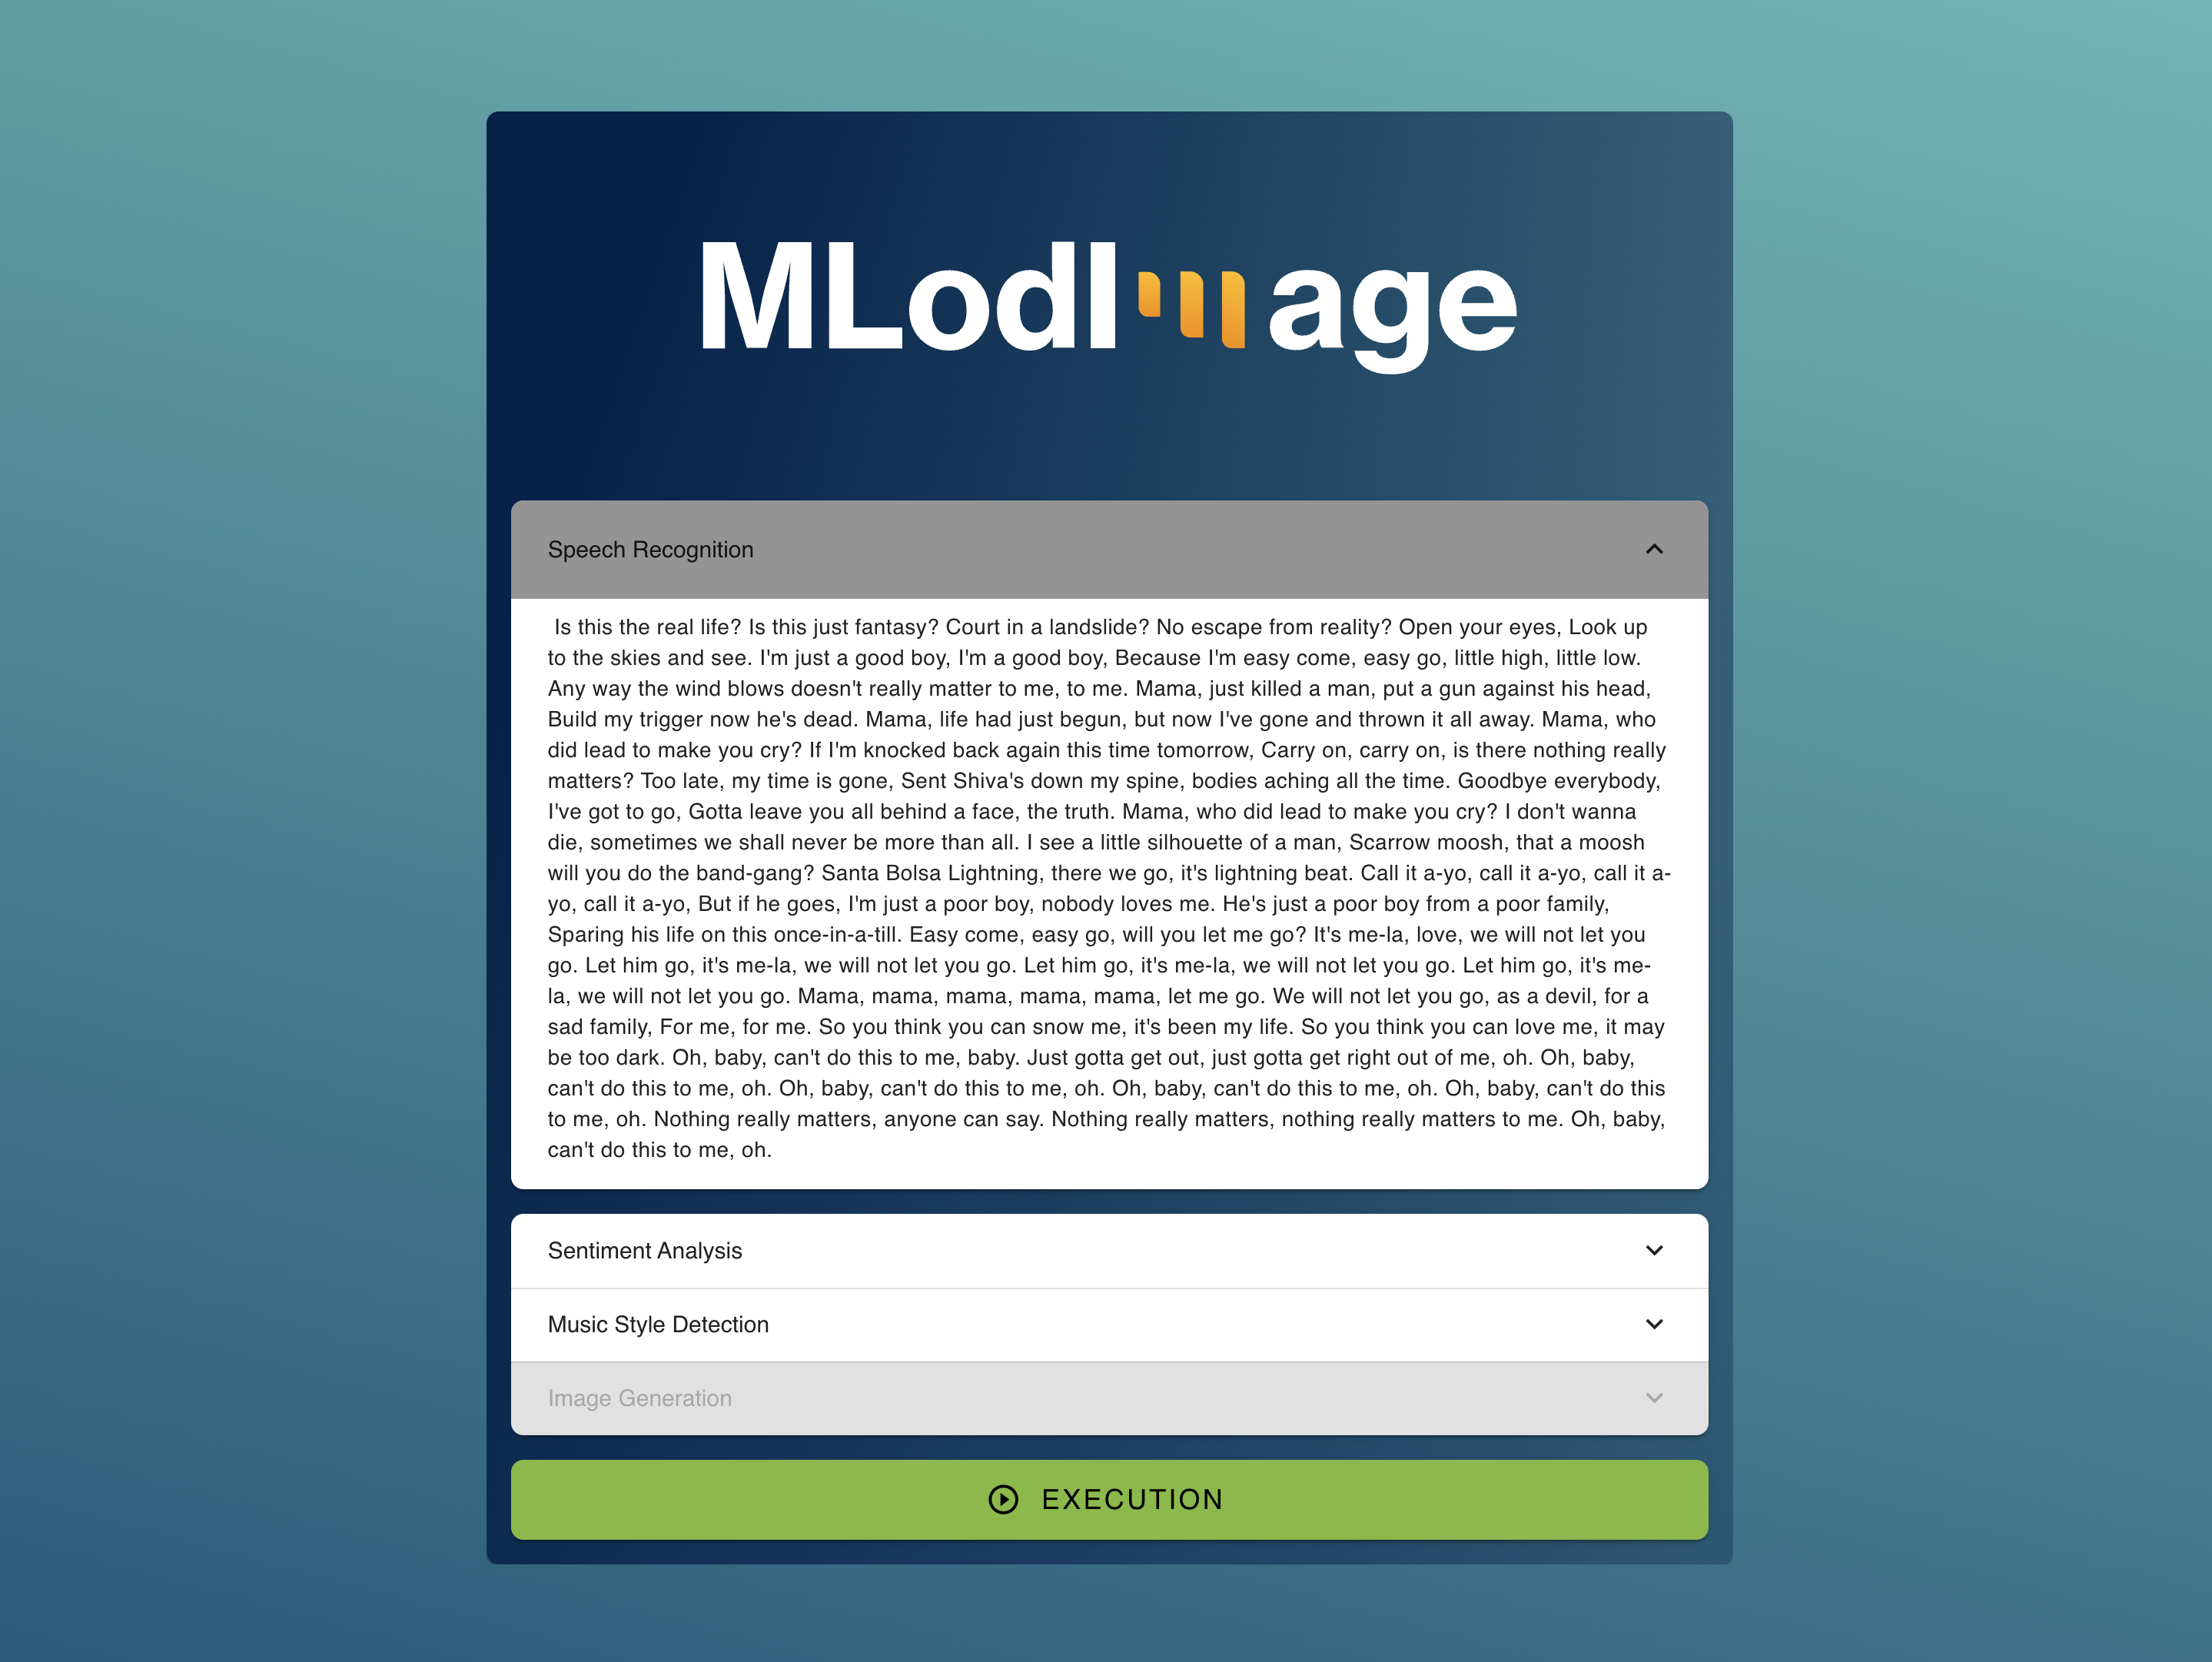
\includegraphics[width=10cm,]{rapport_PI/rsc/webapp_results_tab.png}
        \caption{Web app - Résultats intermédiaires}
        \label{fig:webapp_results_tab}
    \end{center}
\end{figure}

Lorsque l'exécution se termine, on peut voir, en défilant de gauche à droite, trois images qui ont chacune été générées par des modèles différents (figure \ref{fig:webapp_result}). On peut retrouver le nom de ces derniers en haut à droite de chaque image. Il est ensuite possible de télécharger une image via son bouton situé en haut à gauche ou de télécharger les trois d'un coup via le bouton en dessous de l'affichage. L'utilisateur peut remettre l'interface à zéro en appuyant sur le bouton "Reset".

\begin{figure}[H]
    \begin{center}
        \includegraphics[width=10cm,]{rapport_PI/rsc/webapp_result.png}
        \caption{Web app - Résultat final}
        \label{fig:webapp_result}
    \end{center}
\end{figure}

\section{Core Engine}

Le dernier point du projet est la compatibilité avec le Core Engine du CSIA-PME. Ce dernier est un catalogue de micro-services et de pipelines et un des objectifs du projet est de rendre chaque services développé compatible avec la spécification du Centre.

Les différents micro-services ont été, dès le début, développé à l'aide du template fournit sur le Git du projet. Ainsi les services peuvent être enregistrés dans le catalogue, comme le montre la figure \ref{fig:csia_webapp}, et être utilisés via l'interface du CSIA-PME.

\begin{figure}[H]
    \begin{center}
        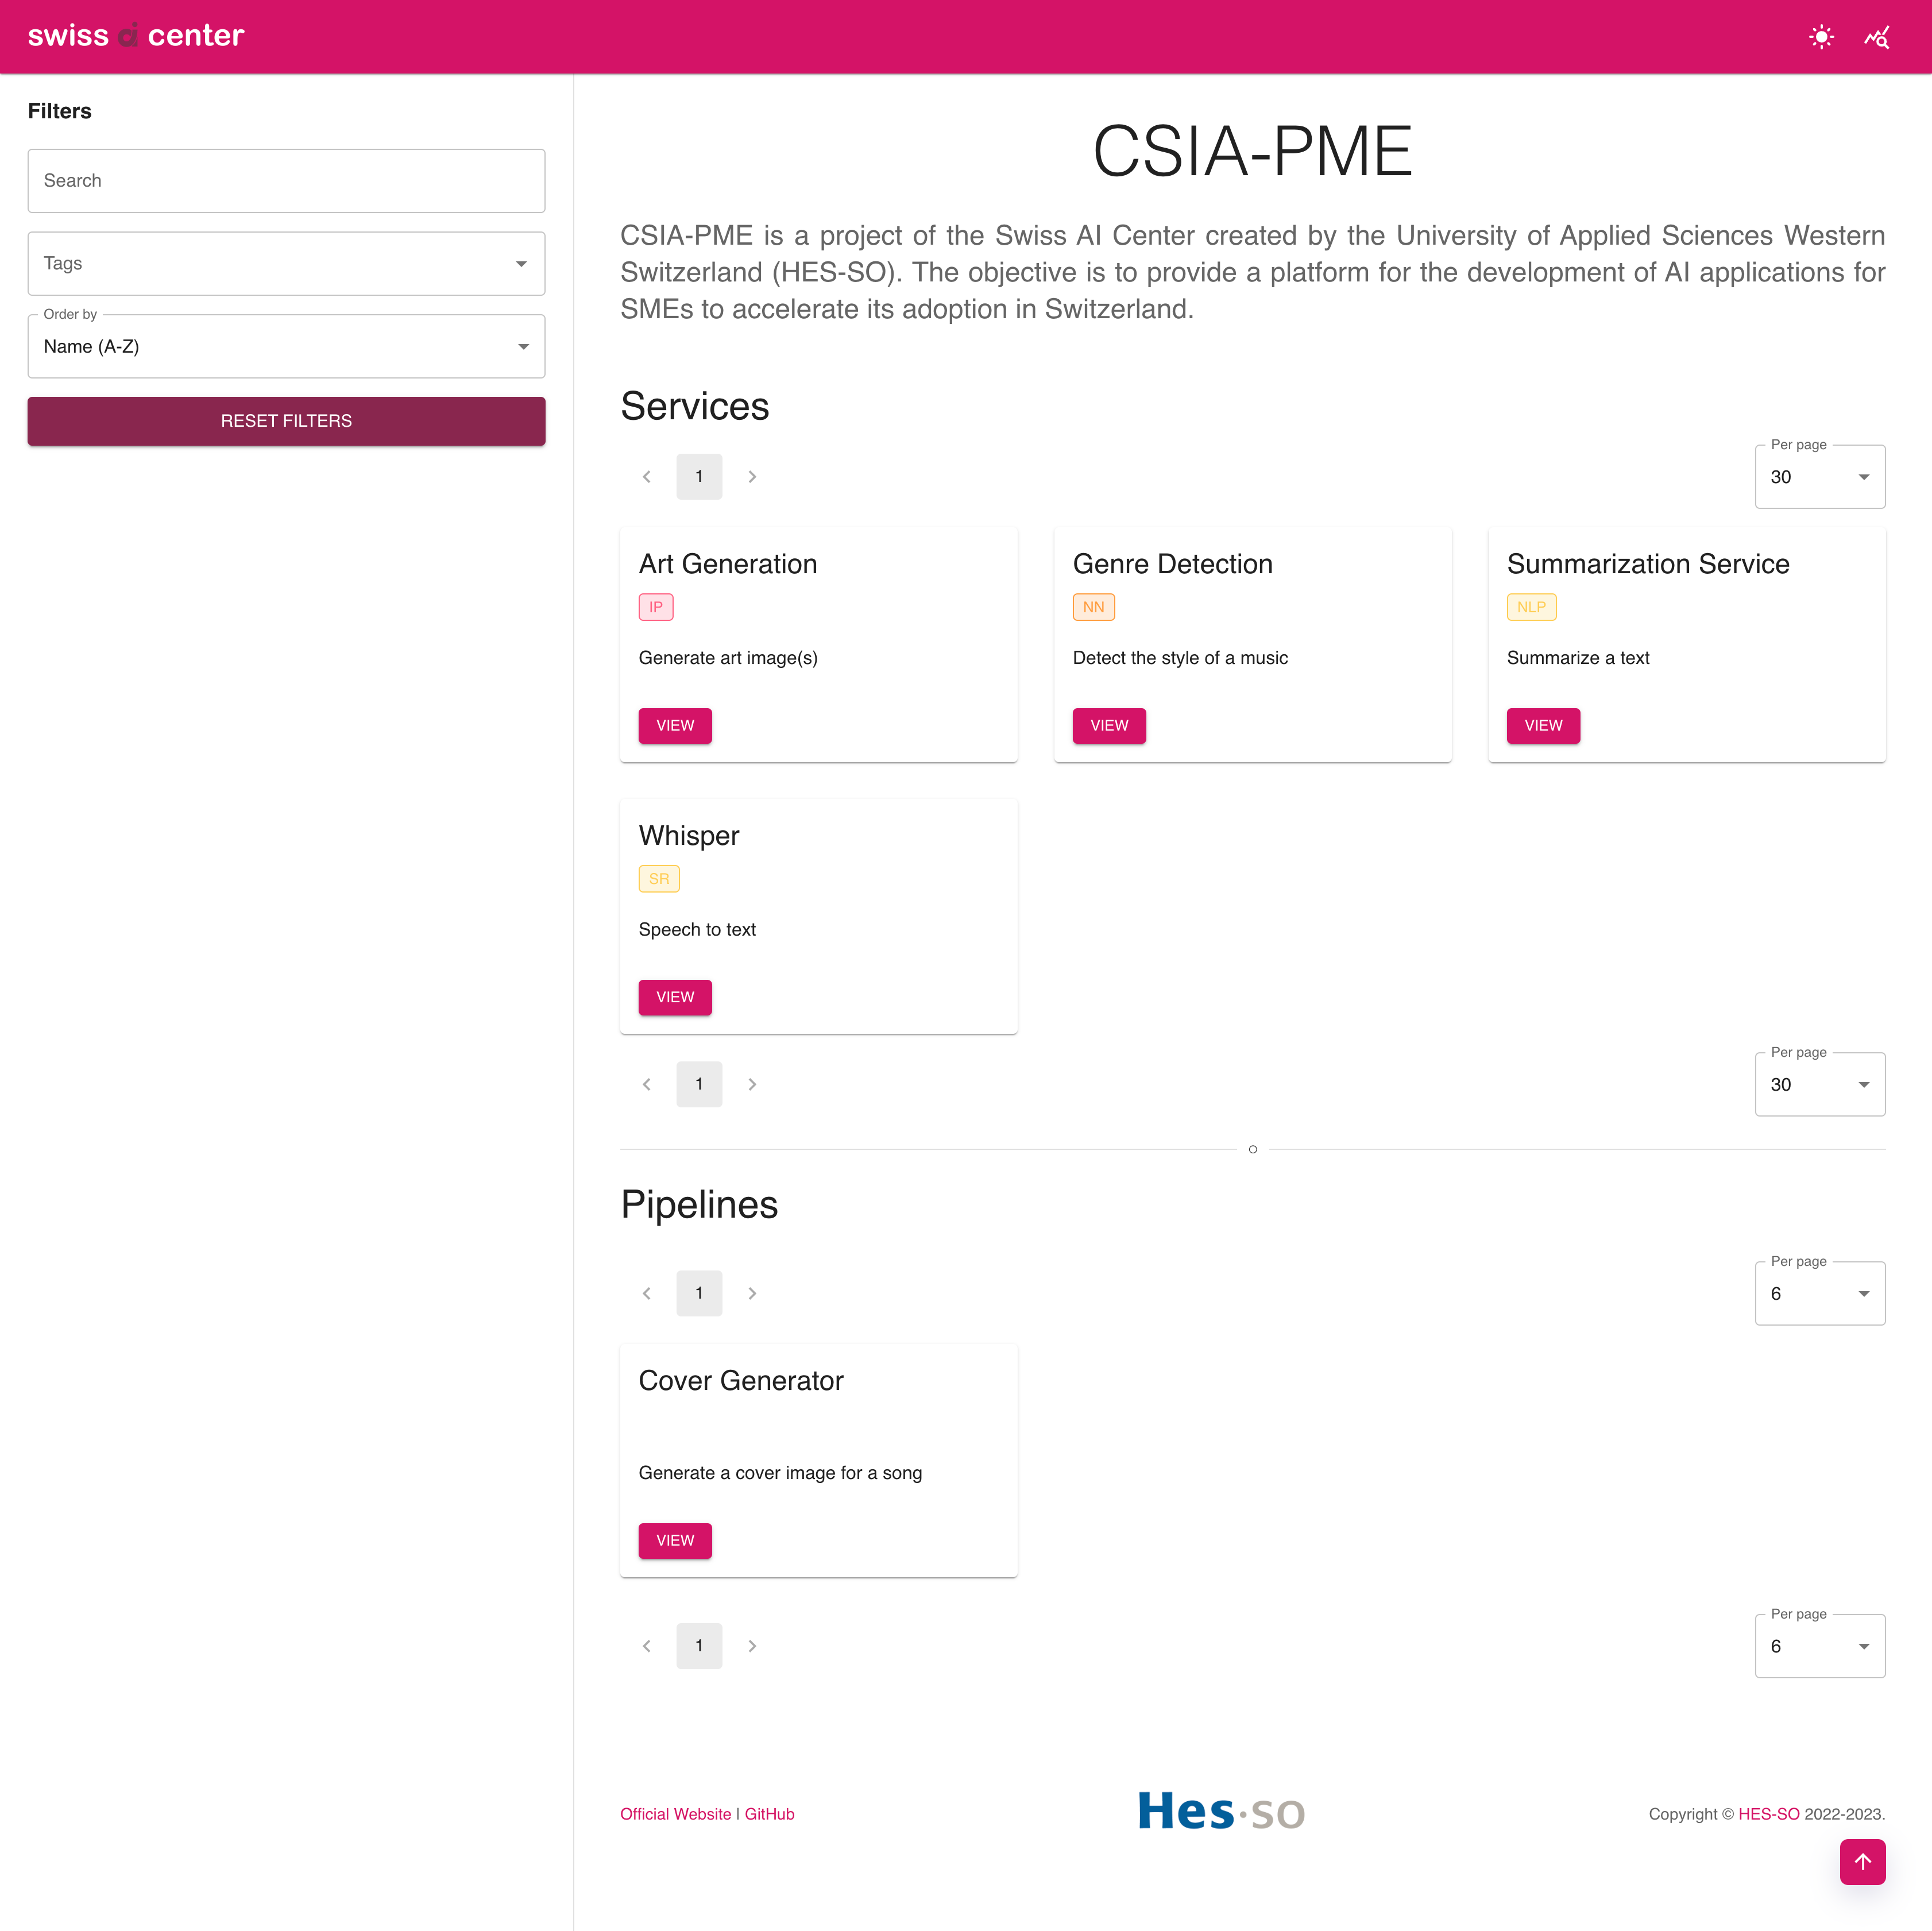
\includegraphics[width=11cm,]{rapport_PI/rsc/csia_webapp.png}
        \caption{CSIA-PME - Web app}
        \label{fig:csia_webapp}
    \end{center}
\end{figure}

Comme l'implémentation des pipelines sur l'Engine du CSIA s'est terminée vers la fin du projet, notre générateur de pochettes peut être ajouté sur le site du centre et peut y être utilisé (figure \ref{fig:csia_pipeline}).

\begin{figure}[H]
    \begin{center}
        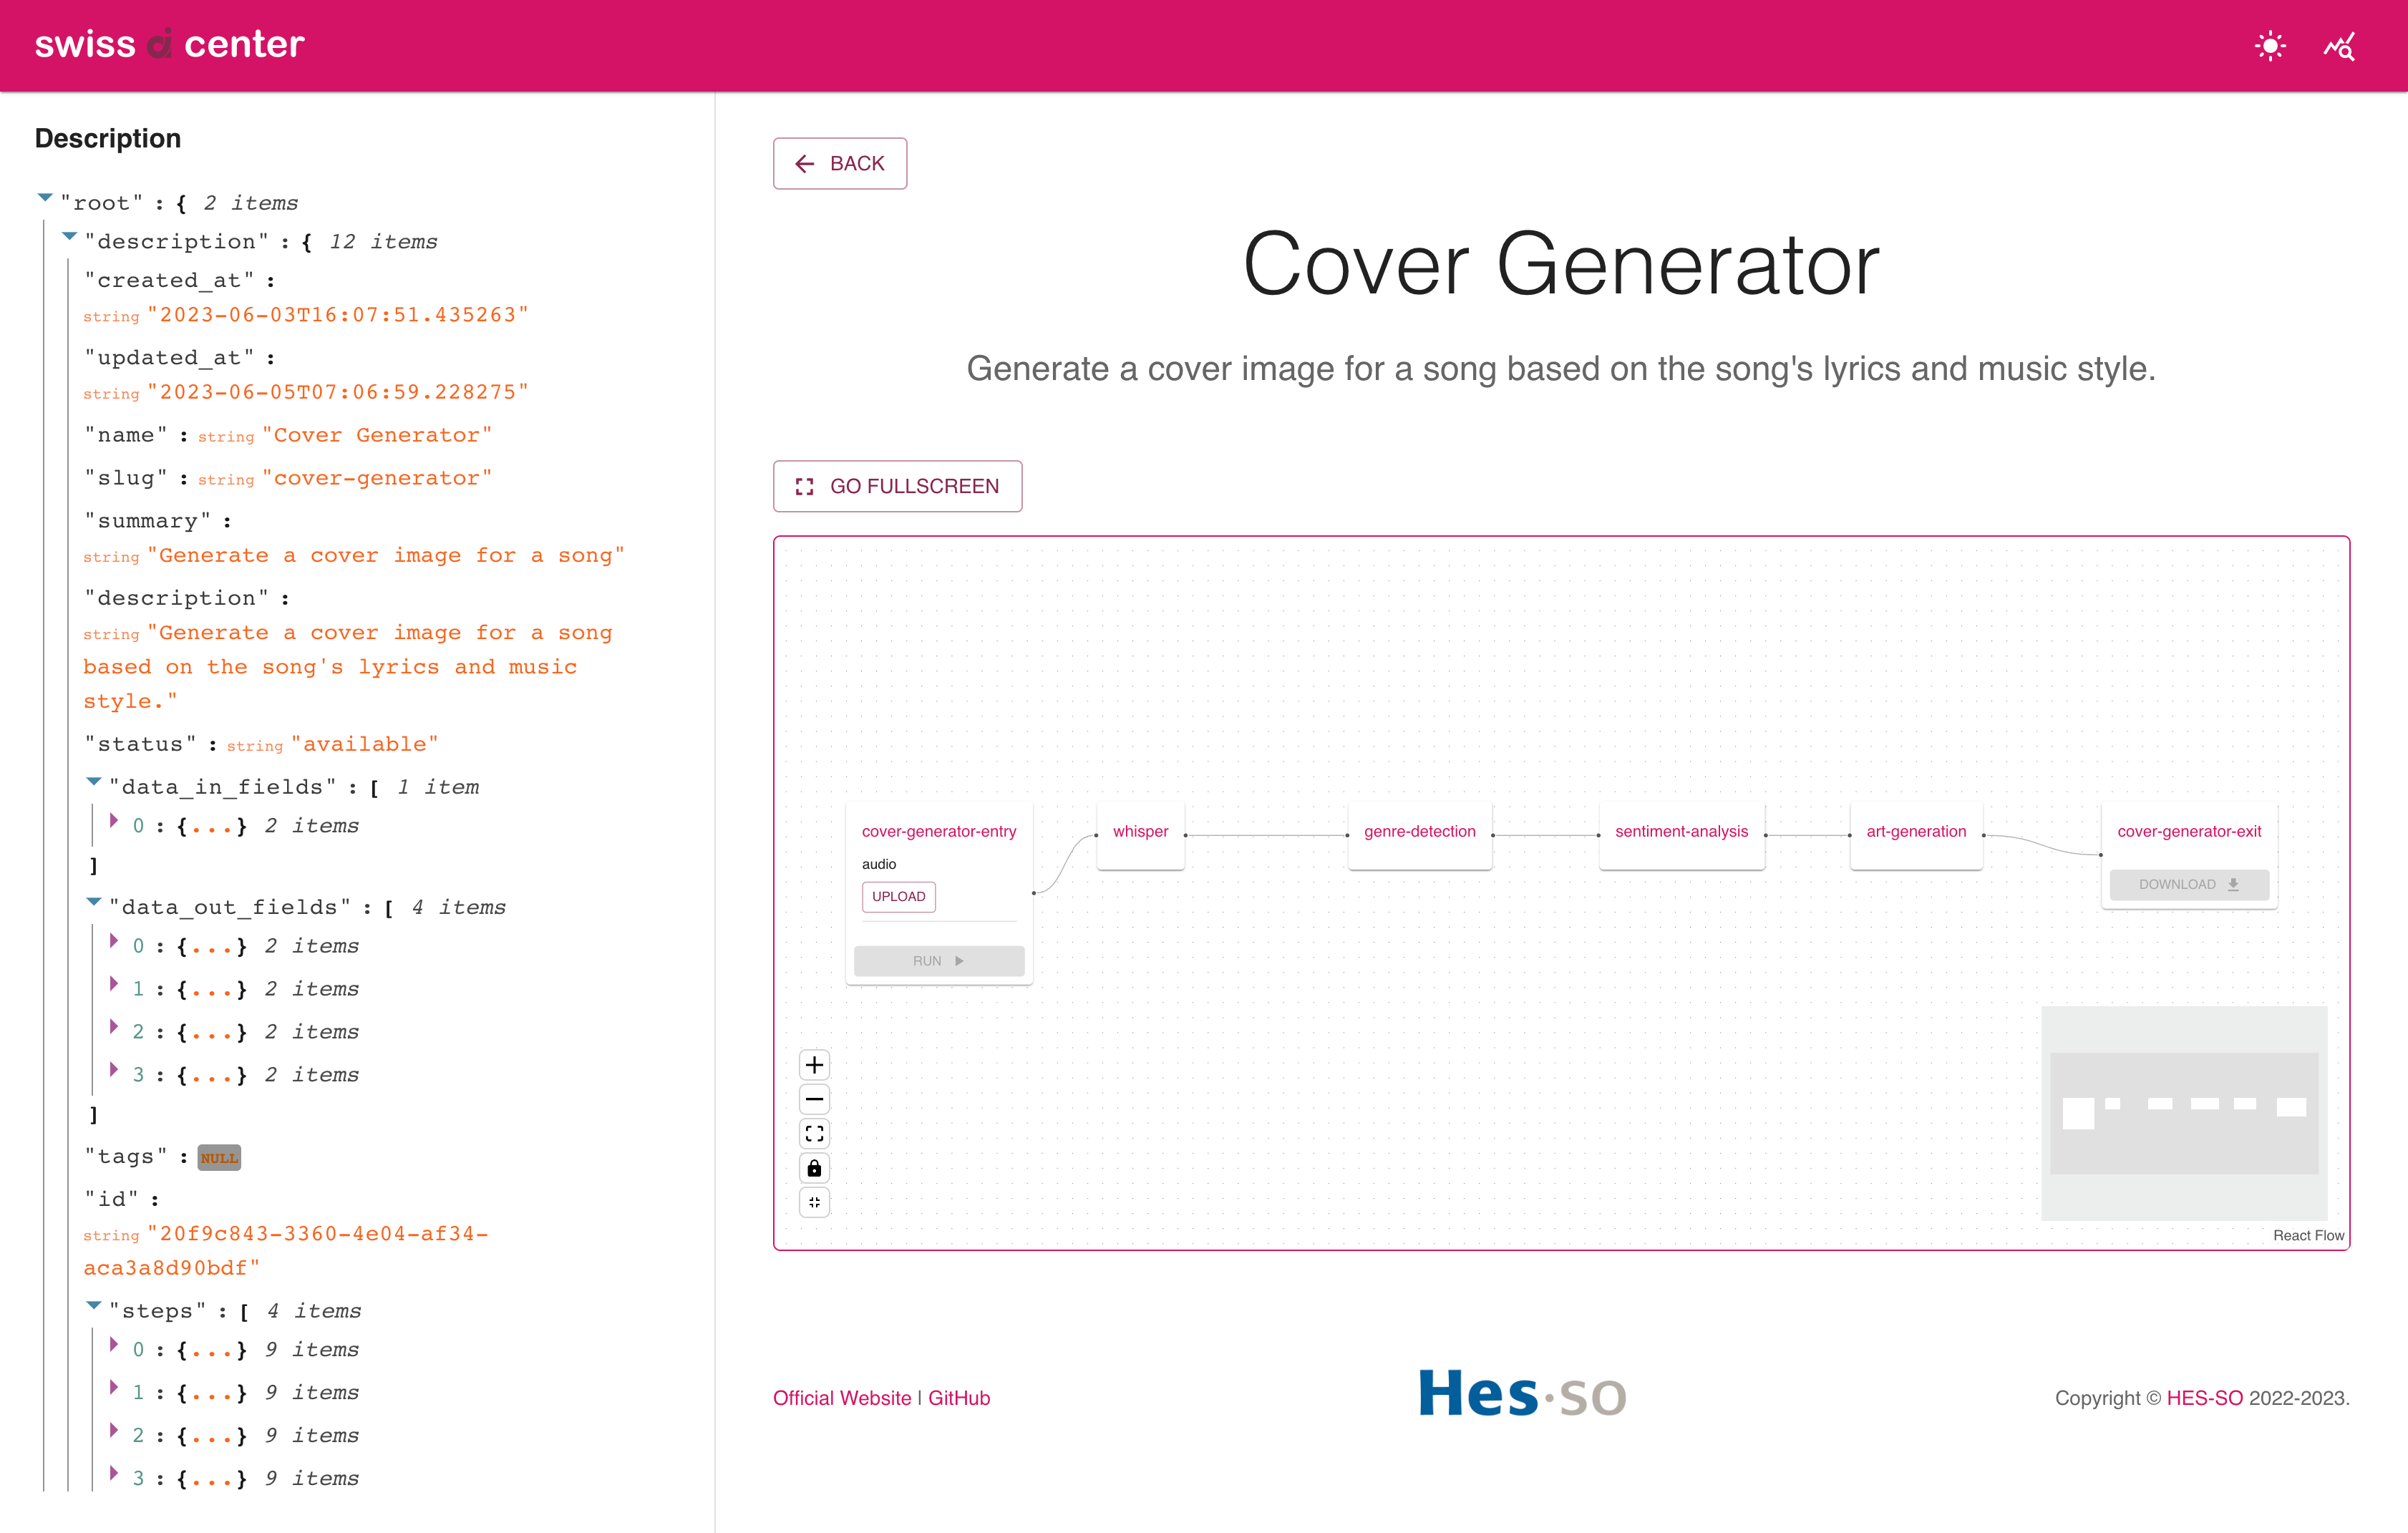
\includegraphics[width=12cm,]{rapport_PI/rsc/csia_pipeline.png}
        \caption{CSIA-PME - Pipeline}
        \label{fig:csia_pipeline}
    \end{center}
\end{figure}

Il y a donc deux interfaces qui permettent d'utiliser nos services.